\chapter{Linear discriminant functions}
\label{cha:linear_discriminant_function}
We can distinguish learning models between \textit{generative learning models} and \textit{discriminative learning models}.
\begin{itemize}
    \item \textbf{Generative learning} assumes knowledge of the distribution governing the data. In essence the purpose of generative models is to model the distribution governing the data. For example, Bayesian network is a generative model since it models the joint probability among the variables in the network. In this manner it is possible to make prediction about the variables in the network. Moreover, with a generative model we can generate new data (samples) according to the distribution.
    
    \item \textbf{Discriminative learning} focuses on directly modeling the discriminant function. For example, for classification, the aim is to directly modeling the decision boundaries rather than inferring them from the modelled data distributions. We use discriminative learning models when we know that the purpose of our application is always to predict the output given the input (e.g. supervised learning). In this case we model the relationship between input and output, without taking into account the underlying generative process. In the context of classification, this means modeling the boundaries directly rather than the data distribution.
\end{itemize}
These distinction is graphically illustrated in Figure \ref{descriminative_generative_11}. In the case of Gaussian classifiers, the aim is to learn a Gaussian probabilistic distribution for each class. At this point, the Gaussian distributions allow to model the relationship between $X$ and $Y$, i.e. the joint probability $P(X,Y) = P(X|Y)P(Y)$, where $P(X|Y)$ are the Gaussian distributions and $Y$ is the set of all possible classes. This kind of model represents the joint probability between input and output. On the other hand, discriminative functions track boundaries between the possible classes. Indeed, in order to make predictions of $Y$ given $X$ it is not necessary to model the full joint probability. We can focus only on learning the boundaries. In essence, we learn a function (\textit{disicriminative function}) $f: X \rightarrow Y$ which directly models $P(Y|X)$.

\begin{figure}
    \centering
    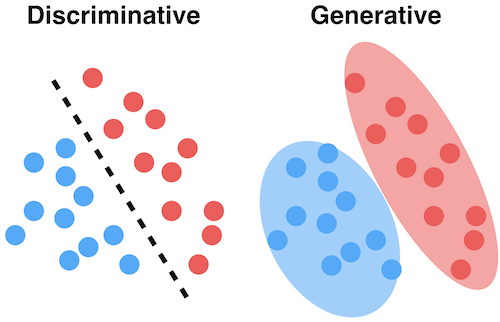
\includegraphics[width=0.5\textwidth]{images/descriminative_generative.png}
    \caption{Discriminative \textit{vs} Generative Models}
    \label{descriminative_generative_11}
\end{figure}

\section{Advantages and disadvantages of discriminative learning}
In the following we discuss about some pros and cons related to the adoption of discriminative learning models. \newline

\textbf{Pros:}
\begin{itemize}
    \item When data are complex, modeling their underlying distribution can be very difficult (e.g. $P(X|Y)$ where $X$ represents high resolution images)
    
    \item If data discrimination is the goal, data distribution modeling is not needed
    
    \item As a consequence we can focus only on learning (using the available training examples) the parameters which are interesting to understand the mapping between input and output
\end{itemize}

\textbf{Cons:}
\begin{itemize}
    \item The learned model is less flexible in its usage. Indeed, discriminative models have fixed input and fixed output.
    
    \item It does not allow to perform arbitrary inference tasks. Really often in these scenarios there is not a precise distinction between inputs and outputs.
    
    \item It is not possible to efficiently generate new data from a certain class.
\end{itemize}

\section{Linear discriminant functions}
A linear discriminative model is a discriminative model which use a linear function to make predictions.\\
The \textit{discriminant function} is a linear combination of example features ($\pmb{x}$).
\begin{equation}
\label{eq:linear_discriminative_function}
    f(\pmb{x}) = \pmb{w}^T \pmb{x} + w_0
\end{equation}
In the formula, $w_0$ is called \textit{bias} or \textit{threshold}. Equation \ref{eq:linear_discriminative_function} is the simplest possible discriminant function. Depending on the complexity of the task and amount of data, it can be the best option available (at least it is the first to try).

\subsection{Linear binary classifier}
In binary classification the predictied class is obtained taking the sign of the linear function.
\begin{equation}
    f(\pmb{x}) = \mathit{sign}(\pmb{w}^T \pmb{x} + w_0)
\end{equation}
The decision boundary, which is a hyperplane ($H$), is achieved when $f(\pmb{x})=0$. \newline

\textbf{Remark:} the weight vector $\pmb{w}$ is orthogonal to the decision hyperplane (Figure \ref{fig:linearBinaryClassifier}). \textbf{Proof:} we take two points on the decision boundary:
$$\forall \pmb{x}, \pmb{x}' : f(\pmb{x}) = f(\pmb{x}') = 0$$
We can replace $f(\pmb{x})$ and $f(\pmb{x}') = 0$ according to Equation \ref{eq:linear_discriminative_function}:
$$\pmb{w}^T \pmb{x} + w_0 = \pmb{w}^T \pmb{x}' + w_0 = 0$$
$$\pmb{w}^T \pmb{x} + w_0 - \pmb{w}^T \pmb{x}' - w_0 = 0$$
$$\pmb{w}^T (\pmb{x} - \pmb{x}') = 0$$
This means that vector $\pmb{w}^T$ and vector $(\pmb{x} - \pmb{x}')$ are orthogonal.

\begin{figure}
    \centering
    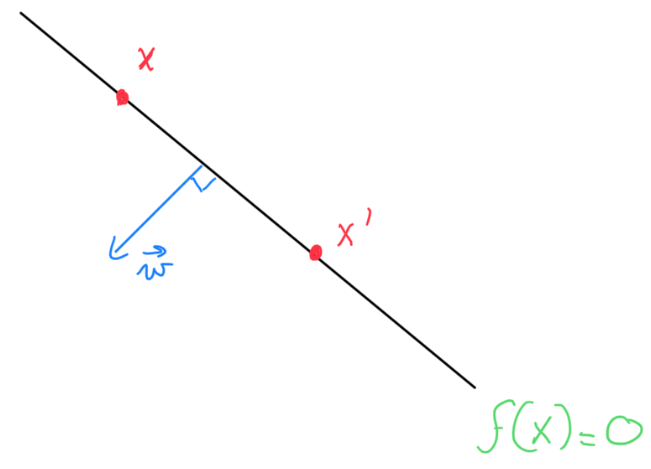
\includegraphics[width=0.5\textwidth]{images/linearBinaryClassifier.png}
    \caption{The weight vector $\pmb{w}$ is orthogonal to the decision hyperplane.}
    \label{fig:linearBinaryClassifier}
\end{figure}

\defi{\textbf{Functional margin}\label{def:functionalMargin}\\
    The value $f(\pmb{x})$ of the function for a certain point $\pmb{x}$ is called \textit{functional margin}. It can be seen as a confidence in the prediction.
}

In a sense, the functional margin represents the margin before predicting the opposite class. The closer $f(\pmb{x})$ is to zero, the smaller the confidence of our prediction.

\defi{\textbf{Geometric margin}\label{def:geometricMargin}\\
    The distance from $\pmb{x}$ to the hyperplane is called \textit{geometric margin}:
    \begin{equation}
        r^x = \frac{f(\pmb{x})}{||\pmb{w}||}
    \end{equation}
    It is a normalize version of the functional margin.
}

\textbf{Remark:} the distance from the origin to the hyperplane is:
\begin{equation}
    r^0 = \frac{f(\pmb{0})}{||\pmb{w}||} = \frac{w_0}{||\pmb{w}||}
\end{equation}

These concepts can be further clarified looking at Figure \ref{fig:linearBinaryClassifier_geometricMargin}. Given an arbitrary point $\pmb{x}$, it can be expressed by its projection on $H$ ($\pmb{x}^p$) plus its distance to $H$ ($r^x$) times the unit vector in that direction ($\frac{\pmb{w}}{||\pmb{w}||}$): $$\pmb{x} = \pmb{x}^p + r^x \frac{\pmb{w}}{||\pmb{w}||}$$

At this point we can replace this value of $x$ into Equation \ref{eq:linear_discriminative_function}:
\begin{align*}
    f(\pmb{x}) = \pmb{w}^T \pmb{x} + w_0 &=\\
    = \pmb{w}^T (\pmb{x}^p + r^x \frac{\pmb{w}}{||\pmb{w}||}) + w_0 &=\\
    = \pmb{w}^T \pmb{x}^p + w_0 + r^x \pmb{w}^T \frac{\pmb{w}}{||\pmb{w}||}
\end{align*}
We can notice that $\pmb{w}^T \pmb{x}^p + w_0 = f(\pmb{x}^p)$. We know that $f(\pmb{x}^p) = 0$ because $\pmb{x}^p$ is on the decision boundary. Moreover:
$$\frac{\pmb{w}^T \pmb{w}}{||\pmb{w}||} = \frac{\pmb{w}^T \pmb{w}}{\sqrt{\pmb{w}^T \pmb{w}}} = \sqrt{\pmb{w}^T \pmb{w}} = ||\pmb{w}||$$
Given these, we can write:
$$f(\pmb{x}) = r^x ||\pmb{w}||$$
$$\frac{f(\pmb{x})}{||\pmb{w}||} = r^x$$

\begin{figure}
    \centering
    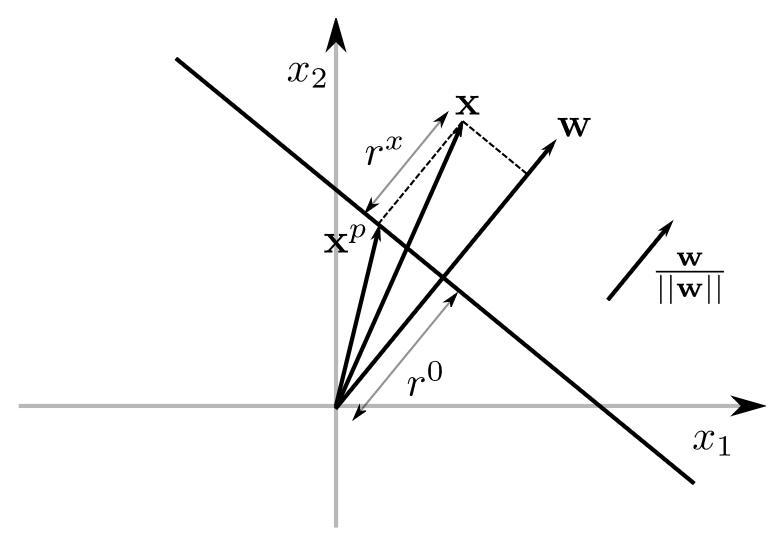
\includegraphics[scale=0.4]{images/linearBinaryClassifier_geometricMargin.png}
    \caption{A point (\pmb{x}) can be expressed by its projection on $H$ plus its distance to $H$ times the unit vector in that direction: $\pmb{x} = \pmb{x}^p + r^x \frac{\pmb{w}}{||\pmb{w}||}$}
    \label{fig:linearBinaryClassifier_geometricMargin}
\end{figure}

\section{Perceptron}
In order to introduce the perceptron, in the following we write about the biological motivation behind this concept.

\subsection{Biological motivation}
The human brain is composed of densely interconnected network of \textit{neurons} (Figure \ref{fig:brainNetwork}). A neuron is made of:
\begin{itemize}
    \item \textit{soma}: a central body containing the nucleus
    \item \textit{dendrites}: a set of filaments departing from the body
    \item \textit{axon}: a longer filament (up to 100 times body diameter)
    \item \textit{synapses}: connections between dendrites and axons from other neurons
\end{itemize}
Electrochemical reactions allow signals to propagate along neurons via axons, synapses and dendrites. Synapses can either \textbf{excite} or \textbf{inhibit} a neuron potential. Each neuron receives (and "accumulates") signals from other neurons. Once a neuron potential exceeds a certain \textbf{threshold}, a signal is generated and transmitted along the axon.

\begin{figure}
    \centering
    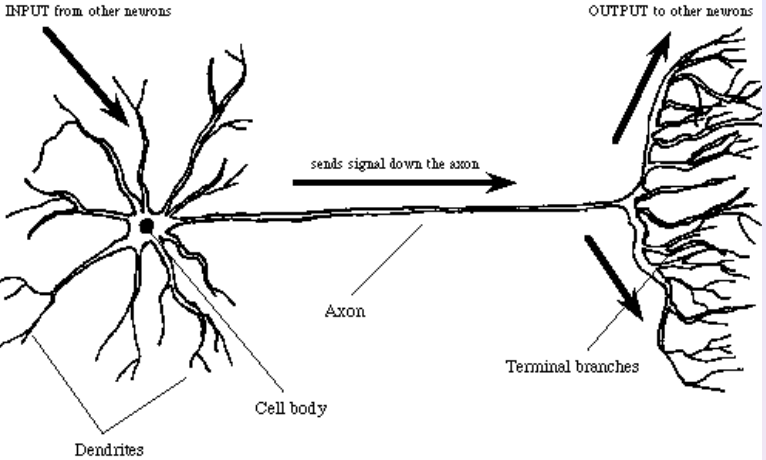
\includegraphics[scale=0.5]{images/brainNetwork.png}
    \caption{The human brain is composed of densely interconnected network of \textit{neurons}.}
    \label{fig:brainNetwork}
\end{figure}

\subsection{Single neuron architecture} 
Mathematically, the neuron structure can be implemented by the \textit{perceptron} (Figure \ref{fig:singleNeuronArchitecture}).
\begin{equation}
    \label{eq:SingleNeuronArchitecture}
    f(x) = \mathit{sign}(\pmb{w}^T \pmb{x} + w_0)
\end{equation}
The function is a linear combination of input features. The coefficients of the linear combination are the weights which can be seen as the synapses. Positive weights excite, negative weights inhibit. The weighted signals are summed up. The result of the summation is processed by an activation function to decide whether to fire or not. In this context "firing or not" means giving output $0$ or $1$. \newline

\textbf{Remark:} we always append to the values $\{x^1 \hdots x^m\}$ a bias $x^0 = 1$.

\begin{figure}
    \centering
    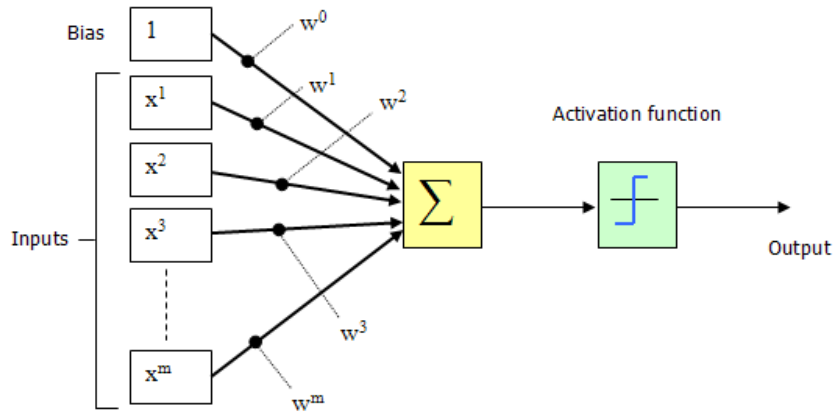
\includegraphics[scale=0.5]{images/singleNeuronArchitecture.png}
    \caption{Single neuron architecture.}
    \label{fig:singleNeuronArchitecture}
\end{figure}

\subsection{Representational power}
A single linear classifier can represent \textit{linearly separable} sets of examples (e.g. primitive boolean functions (AND, OR, NAND, NOT) - Figure \ref{fig:andPerceptron} and Figure \ref{fig:orPerceptron}). 

\begin{figure}
    \centering
    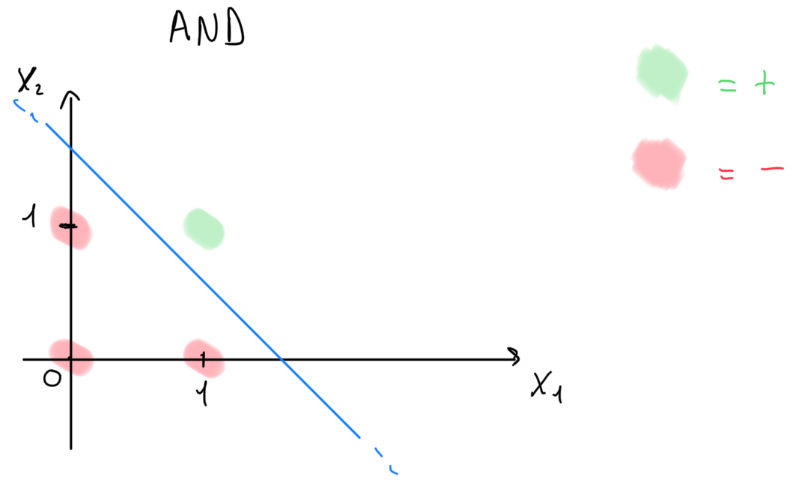
\includegraphics[scale=0.5]{images/andPerceptron.png}
    \caption{A single linear classifier can represent \textit{linearly separable} sets of examples. For example the AND boolean function.}
    \label{fig:andPerceptron}
\end{figure}

\begin{figure}
    \centering
    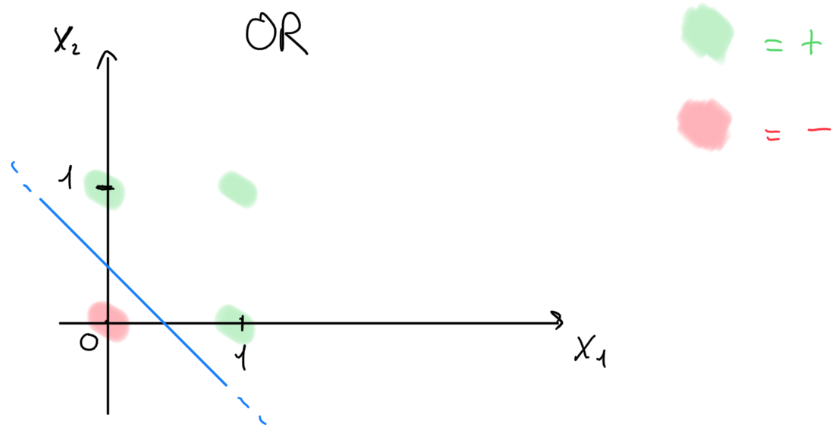
\includegraphics[scale=0.5]{images/orPerceptron.png}
    \caption{A single linear classifier can represent \textit{linearly separable} sets of examples. For example the OR boolean function.}
    \label{fig:orPerceptron}
\end{figure}

A linear classifier can not learn more complex boolean formula like the XOR (Figure \ref{fig:xorPerceptron}). \newline

\begin{figure}
    \centering
    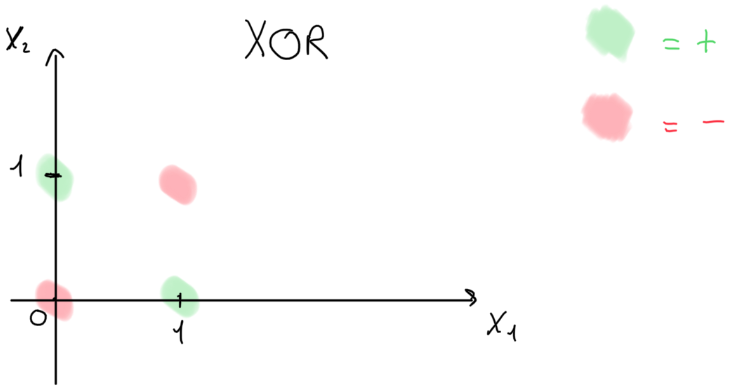
\includegraphics[scale=0.5]{images/xorPerceptron.png}
    \caption{A linear classifier can not learn more complex boolean formula like the XOR.}
    \label{fig:xorPerceptron}
\end{figure}

However, the XOR can be represented in terms of AND and OR:
$$x_1 \oplus x_2 = (x_1 \wedge \Bar{x_2}) \vee (\Bar{x_1} \wedge x_2)$$
At this point $A=(x_1 \wedge \Bar{x_2})$ and $B=(\Bar{x_1} \wedge x_2)$ and $C = A \vee B$ can be represented by a neuron. In particular the input of neuron $C$ are the output of the neurons $A$ and $B$. This means that the XOR can be learnt by a network with two layers. \newline

In general, any logic formula $\phi$ can be written in DNF (disjunctive normal form) or CNF (conjunctive normal form). This means that any logic formula can be represented and learnt by a network of two levels of perceptrons. Unfortunately, it is extremely expensive to represent complex logic formula with two levels of perceptron. \newline

\textbf{Problems}
\begin{itemize}
    \item \textit{non-linearly separable} sets of examples cannot be separated
    \item representing complex logic formulas can require a number of perceptrons exponential in the size of the input. Having an exponential number of perceptron is definitely prohibitive for learning. This models are usually referred to as \textit{shallow models}. The solution is to build deeper models with several perceptron layers. 
\end{itemize}

It is useful to write down Equation \ref{eq:SingleNeuronArchitecture} in a shorter way. To do this, \textit{augmented/weight vectors} are used. The idea is to incorporate the bias in the augmented vector.
\begin{equation}
    f(x) = \mathit{sign}(\pmb{\hat{w}}^T \pmb{\hat{x}})
\end{equation}

\begin{align}
    \pmb{\hat{w}} =
    \begin{pmatrix}
        w_0 \\
        \pmb{w}
    \end{pmatrix}
\end{align}

\begin{align}
    \pmb{\hat{x}} =
    \begin{pmatrix}
        1 \\
        \pmb{x}
    \end{pmatrix}
\end{align}

For the sake of brevity, we skip the hat over $\pmb{x}$ and $\pmb{w}$ in the following, replacing the search for weight vector + bias with the search for the augmented weight vector.

\section{Parameter learning}
Similarly to what we have studied for maximum likelihood for probability distributions, we need to find a function of the parameters to be optimized. A reasonable function is the measure of the error on the training set $\mathcal{D}$. This function is called \textit{loss function} and it compares the ground truth with the output of our model. In few words, $l(y, f(\pmb{x}))$ represents the loss that we have to pay for predicting $f(\pmb{x})$ instead of $y$. As a consequence, the loss function is something to be minimized.
\begin{equation}
    \label{eq:parameterLearning_errorMinimization}
    E(\pmb{w}; \mathcal{D}) = \sum_{(\pmb{X},y) \in \mathcal{D}} l(y, f(\mathcal{x}))
\end{equation}
Finding the parameters to minimize the error function can easily lead to overfitting. However, keep in mind that linear classifier are simple models less prone to overfitting with respect to deep neural networks.

\subsection{Gradient descent}
The common approach to minimize the error function is the \textit{gradient descent}. In the context of optimization problems, the interesting points are where the gradient of the function becomes zero. Unfortunately, once we have this equation, there is no closed formula to solve and get the parameters. In order to face this situation we rely on gradient descent approach in order to progressively find a good local minima of the error function.\\
Gradient descent works as follows:
\begin{enumerate}
    \item initialize $\pmb{w}$ (e.g. $\pmb{w}=0$) (randomly)
    
    \item iterate until gradient is approximately zero:
    \begin{equation}
        \label{eq:gradient_descent}
        \pmb{w} = \pmb{w} - \eta \nabla E(\pmb{w}; \mathcal{D})
    \end{equation}
\end{enumerate}

\textbf{Remark:} the gradient points to the maximum of the function. As a result we have to explore the function in the opposite direction $- \eta \nabla E(\pmb{w}; \mathcal{D})$.

\begin{itemize}
    \item $\eta$ is called \textit{learning rate} and controls the amount of movement at each gradient step. In essence, the gradient gives us information about the \textit{direction} while the learning rate quantifies the \textit{size of the step} along the suggested direction.
    
    \item the algorithm is guaranteed to converge to a local optimum of $E(\pmb{w}; \mathit{D})$ (for small enough $\eta$)
    
    \item too low $\eta$ implies slow convergence. On the other hand, with too high values of $\eta$ we end up oscillating.
    
    \item techniques exist to adaptively modify $\eta$
\end{itemize}

In the case of the linear classifier, the misclassification loss is picewise constant and so it is a poor candidate for gradient descent. Indeed, applying gradient descent with a function like the one represented in Figure \ref{fig:scalini} the gradient is either 0 or it does not exist. In order to apply gradient descent approach, we need functions with a smoother behaviour. As a consequence we adopt a different training rule, the \textit{perceptron training rule}. Following this approach, the error is the sum of the functional margins ($f(\pmb{x})$) of incorrectly classified examples:
\begin{equation}
    \label{perceptronTrainingRule1}
    E(\pmb{w}; \mathcal{D}) = \sum_{(\pmb{X},y) \in \mathcal{D}_E} -y f(\pmb{x}))
\end{equation}
where $\mathcal{D}_E$ is the set of current training errors for which:
$$y f(\pmb{x}) \leq 0$$
Indeed, we do not consider the right predictions but we take into consideration only the wrong predictions. \newline

With this approach we are taking into consideration the confidence of our predictions. For this reason, we typically refer to this kind of loss functions as \textit{confidence loss}. We compare the confidence of the prediction with respect to the actual class. \newline

\textbf{Remark:} We write $ - y f(\pmb{x})$ because we want to maximize the confidence of the correct predictions (or analogously minimize the incorrect predictions characterized by high confidence). \newline

\begin{figure}
    \centering
    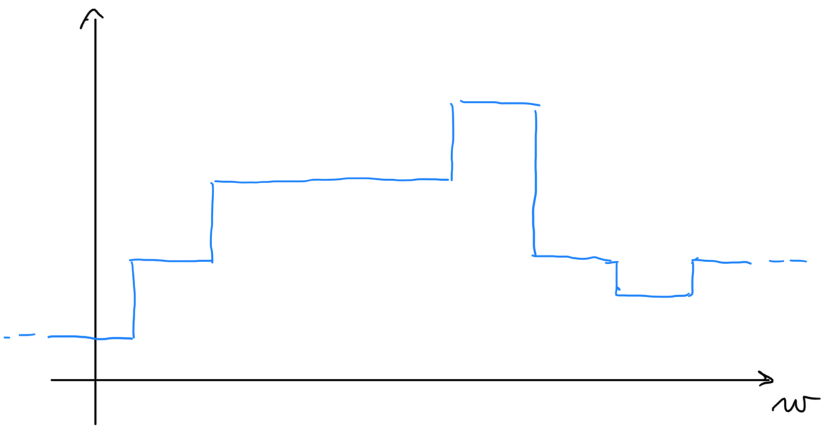
\includegraphics[width=\textwidth]{images/gradini.png}
    \caption{The misclassification loss is picewise constant and so it is a poor candidate for gradient descent.}
    \label{fig:scalini}
\end{figure}

We apply gradient descent on Equation \ref{perceptronTrainingRule1}:
\begin{align*}
    \nabla E(\pmb{w};\mathcal{D}) &=\\
    \nabla \sum_{(\pmb{X}, y) \in \mathcal{D}_E} -y f(\pmb{x}) &=\\
    \nabla \sum_{(\pmb{X}, y) \in \mathcal{D}_E} -y (\pmb{w}^T \pmb{x})
\end{align*}
The gradient of $\pmb{w}^T \pmb{x}$ with respect to $\pmb{w}$ is just $\pmb{x}$.
\begin{align*}
    \nabla E(\pmb{w};\mathcal{D}) &=\\
    \nabla \sum_{(\pmb{X}, y) \in \mathcal{D}_E} -y (\pmb{w}^T \pmb{x}) &=\\
    \sum_{(\pmb{X}, y) \in \mathcal{D}_E} -y \pmb{x}
\end{align*}
The amount of update is:
$$- \eta \nabla E(\pmb{w}; \mathcal{D}) = \eta \sum_{(\pmb{X},y) \in \mathcal{D}_e} y \pmb{x}$$
This last is the update of $\pmb{w}$ at each iteration.

\subsection{Stochastic perceptron training rule}
Following the approach we have presented so far, in order to update the vector of the weights, we have to iterate over all the training set at each iteration to compute the gradient of the error for each example. This results in slow convergence if we have many examples (e.g. deep learning). \textit{Stochastic perceptron training rule} is an alternative to this model.

\begin{enumerate}
    \item Initialize weights randomly
    \item Iterate until all examples are correctly classified:
    \begin{enumerate}
        \item for each incorrectly classified training example ($\pmb{x}$,y) update the weight vector:
        $$\pmb{w} \leftarrow \pmb{w}+\eta y \pmb{x}$$
    \end{enumerate}
\end{enumerate}

\textbf{Remark:} the update formula $\pmb{w} \leftarrow \pmb{w}+\eta y \pmb{x}$ is the same as before but there is not the summation over all the training data. We update the weight vector considering only one example. \newline

With this method, we make a gradient step for each training error, rather than on the sum of them in \textit{batch} learning. In this way, each gradient step is very fast. Moreover, stochasticity can sometimes help to avoid local minima (i.e. it could be more robust), being guided by various gradients for each training example (which won't have the same local minima in general). At each iteration we compute the gradient on a different error function. Following this approach, we stochastically optimize the error function. \newline

\textbf{Remark:} instead of considering one single example at each iteration, some implementations of stochastic gradient discent consider a \textit{minibatch} of training data.

\section{Perceptron regression}
Linear models are not used only for linear classification but also for \textit{linear regression}. \newline

Let $X \in \R^n \times \R^d$ be the input training matrix (i.e. $X = \begin{bmatrix} \pmb{x}^1 \hdots \pmb{x}^n \end{bmatrix}^T$ for $n=|\mathcal{D}|$ and $d=|\pmb{x}|$).\\
Let $\pmb{y} \in \R^n$ be the output training matrix (i.e. $y_i$ is output for example $\pmb{x}^i$) \newline

Regression learning could be stated as a set of linear equations:
\begin{equation}
    X \pmb{w} = \pmb{y}
\end{equation}
Giving as solution:
\begin{equation}
    \pmb{w} = X^{-1} \pmb{y}
\end{equation}

Unfortunately, this approach does not work:

\begin{itemize}
    \item $X$ is not square in general because not necessarily the number of examples is equal to the number of features. In general, matrix $X$ is rectangular, usually more rows than columns
    
    \item System of equations is overdetermined (more equations than unknowns)
    
    \item No exact solution typically exists
\end{itemize}

So, even if the matrix is square, it is not typically invertible. However, our aim is not necessarily to solve the system of equation exactly. It is enough to do the best that we can. Again, we are going to minimize an error function. When dealing with regression and loss minimization, the most common error function which is considered is the \textit{mean squared error} (MSE).
\begin{equation}
    E(\pmb{w}; \mathcal{D}) = \sum_{(\pmb{X},y) \in \mathcal{D}} (y-f(\pmb{x}))^2 = (\pmb{y}-X\pmb{w})^T (\pmb{y} - X \pmb{w})
\end{equation}
For this equation, there is a closed form solution. Moreover, it can also be always solved by gradient descent. This latter approach can be faster. \newline

\textbf{Remark:} Mean squared error can also be used as a classification loss.

\subsection{Closed form solution}
In order to calculate a closed form solution to our problem, the idea is to compute the gradient and make it equal to zero.
\begin{align*}
    \nabla E(\pmb{w}; \mathcal{D}) &=\\
    \nabla (\pmb{y}-X \pmb{w})^T (\pmb{y} - X \pmb{w}) &=\\
    2(\pmb{y}-X \pmb{w})^T (-X) = 0 \\
    -2 \pmb{y}^T X + 2\pmb{w}^T X^T X = 0 \\
    \pmb{w}^T X^T X = \pmb{y}^T X \\
    (\pmb{w}^T X^T X)^T = (\pmb{y}^T X)^T \\
    X^T X \pmb{w} = X^T \pmb{y} \\
    \pmb{w} = (X^T X)^{-1} X^{T} \pmb{y}
\end{align*}

\textbf{Remark:} $\pmb{w}$ is a column vector. \newline

$(X^T X)^{-1} X^{T}$ is a pseudo inverse which is called \textit{left-inverse}. \newline

\textbf{Remark:}
\begin{itemize}
    \item The left-inverse exists provided $(X^T X)\in \R^{d \times d}$ is full rank, otherwise we can't invert it. If $(X^T X)$ is not full rank is because features are linearly dependent. In order to make it full rank, we just remove the redundant features. In this way, all the features are linearly independent and $(X^T X)$ is full rank.
    
    \item If $X$ is square and nonsingular (i.e. invertible), inverse and left-inverse coincide ($(X^T X)^{-1} X^{T} = X^{-1}$) and the MSE solution corresponds to the exact one.
    $$\pmb{w} = X^{-1} \pmb{y}$$
    So, if there is an exact solution, MSE finds it, otherwise it will provide an approximation which minimizes the squared error.
\end{itemize}

In a context with a lot of features, inverting $(X^T X)$ could be very expensive. As a result, instead of solving the equation with the gradient equal to zero, as an alternative, we can compute the gradient and perform gradient descent. For a single weight, the gradient step is computed as illustrated in Figure \ref{fig:perceptronRegressionGradientDescent}. TODO: copiare la formula dell'immagine.

\begin{figure}
    \centering
    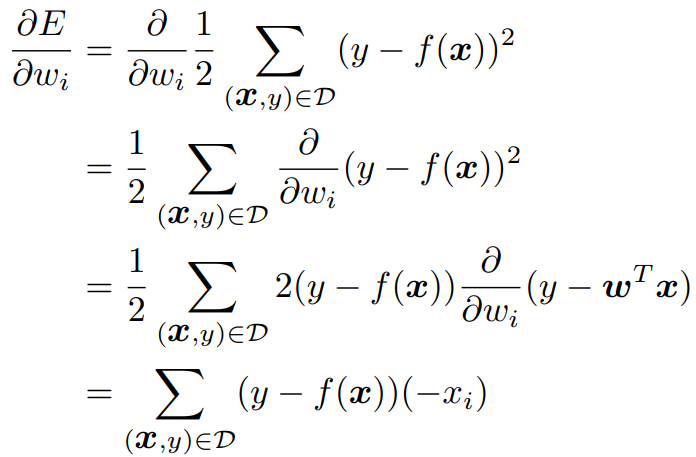
\includegraphics[scale=0.4]{images/perceptronRegressionGradientDescent.png}
    \caption{Solving perceptron regression with gradient descent.}
    \label{fig:perceptronRegressionGradientDescent}
\end{figure}

\section{Multiclass classification}
All the methods illustrated in this section, solve \textit{multiclass classification} by means of combination of binary classification tasks. \newline

\textbf{Remark:} the distinction between multiclass classification and binary classification is necessary in the case of discriminant models. On the other hand, in the generative model domain (e.g. Naive Bayes), there is not a different solution between binary classification and multiclass classification.

\subsection{ONE vs ALL}
The idea of this multiclass classification solution is to learn one binary classifier for each class such that:
\begin{itemize}
    \item positive examples are examples of the class
    \item negative examples are examples of all other classes
\end{itemize}

At this point we have a model with $m$ decision hyperplanes, one per class. Each classifier provides a confidence (score), and we take the class with maximal score. Figuratively, it is as if each classifier votes a class. More formally, the model predicts a new example in the class with maximum functional margin. \newline

Decision boundaries for which $f_i(\pmb{x}) = f_j(\pmb{x})$ are pieces of hyperplanes such that the confidence for class $i$ is equal to the confidence for class $j$. In these configurations, we do not know which of the two classes to choose.
$$\pmb{w}_i^T \pmb{x} = \pmb{w}_j^T \pmb{x}$$
$$(\pmb{w}_i - \pmb{w}_j)^T \pmb{x} = 0$$
From this last equation we observe that the boundary is actually a hyperplane (Figure \ref{fig:oneVsAllMulticlassClassification}).

\begin{figure}
    \centering
    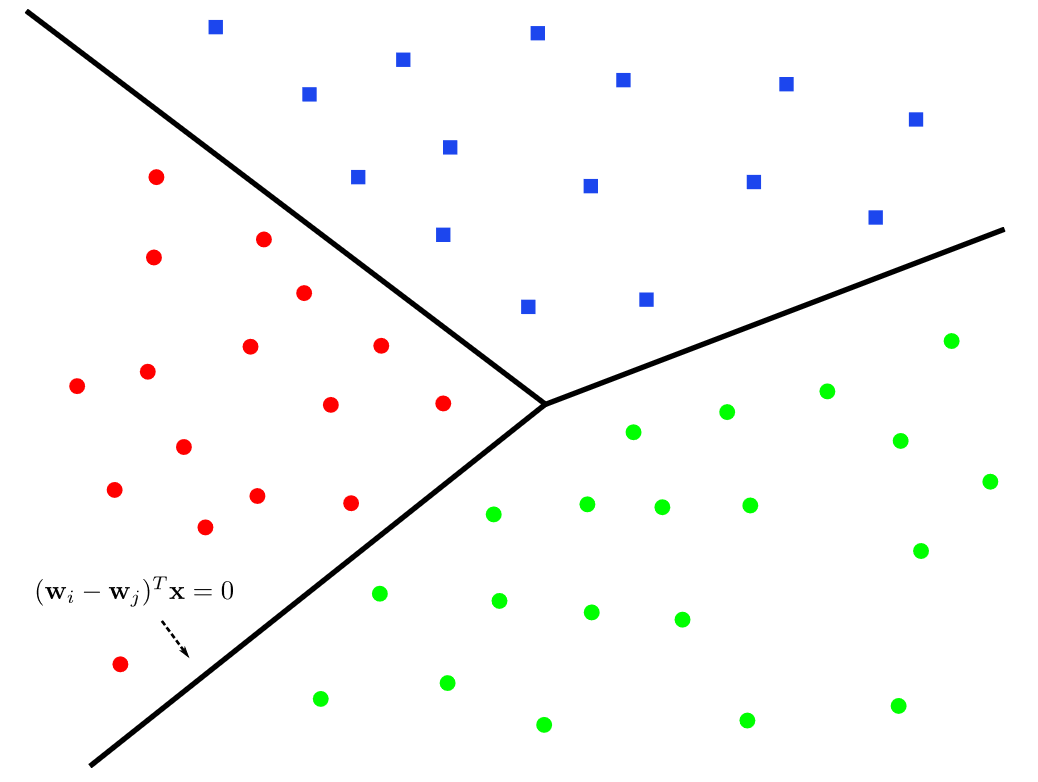
\includegraphics[scale=0.3]{images/oneVsAllMulticlassClassification.png}
    \caption{Multiclass classification decision boundaries.}
    \label{fig:oneVsAllMulticlassClassification}
\end{figure}

\subsection{ONE vs ALL (all pairs)}
The aim of this multiclass classification solution is to learn one binary classifier for each pair of classes:
\begin{itemize}
    \item positive examples from one class
    \item negative examples from the other
\end{itemize}
If there are $m$ classes, there will be $\frac{m(m-1)}{2}$ binary classifier. The model predicts a new example in the class winning the largest number of pairwise classifications as in a tournament.

\subsection{ONE vs ONE - ONE vs ALL comparison}
In ONE vs ALL we have to train $m$ classifiers each with all examples. On the other hand, in ONE vs ONE we have to train $\mathcal{O}(m^2)$ classifiers, each with much fewer examples (only the examples of the two classes). If the training procedure complexity is high with respect to the number if examples, all pairs is faster.

\section{Generative linear classifiers}
What kind of generative models produce linear classifiers? At the beginning of this section, we write about \textit{Gaussian classifier}: we have a Gaussian distribution $P(\pmb{x}|y)$ for each class. The task is to compute the posterior $P(y | \pmb{x})$. In the case of Gaussian distributions, linear decision boundaries are obtained when covariance is shared among classes ($\Sigma_i = \Sigma$). This defines a general spread in the space which does not depend on the class. So, only under this assumption the Gaussian classifier becomes a linear classifier. \newline

\textbf{Remark:} Gaussian has the exponential in its formulation, so we typically adopt log-linear Gaussian classifiers. Log-linear classifiers are characterized by the same expressive capability with respect to linear classifiers since the logarithm is a monotonic function. \newline

Another generative model which is also linear is Naive Bayes classifier. In this case, it is required to assume that all features are independent one with respect to the other given the class.
\begin{align*}
    f_i(\pmb{x}) = P(\pmb{x} | y_i) P(y_i) &= \\
    = \prod_{j=1}^{|\pmb{x}|} P(x_j | y_i) P(y_i) &= \\
    = \prod_{j=1}^{|\pmb{x}|} \prod_{k=1}^{K} \theta_{ky_i}^{z_k(x[j])} \frac{|\mathcal{D}_i|}{|\mathcal{D}|} &= \\
    = \prod_{k=1}^{K} \theta_{ky_i}^{N_{k\pmb{x}}} \frac{|\mathcal{D}_i|}{|\mathcal{D}|}
\end{align*}
where $N_{k\pmb{x}}$ is the number of times feature $k$ (e.g. a word) appears in $\pmb{x}$. \newline

\textbf{Remark:}
\begin{itemize}
    \item $\prod_{j=1}^{|\pmb{x}|}$ product over all the possible features
    
    \item $\prod_{k=1}^{K}$ :  $x_j$ is a discrete variable with $k$ possible values
    
    \item $z_k(x[j])$ is a hot encoding of a categorical variable (a categorical variable is a variable which can be represented as a hot encoding). $z_k(x[j])=1$ if the variable takes the $k$ value and zero otherwise
    
    \item $\theta_{ky_i}$ parameter of the kth value for $y_i$ class. It is the probability that feature $k$ of $x_j$ is true given $y_i$. In essence $\theta_{ky_i}$ is raised to the power of 1 when $x_j$ has the kth feature, otherwise $\theta_{ky_i}$ is raised to the power of 0. (Figure \ref{fig:parameterOfTheKthValueForYiClass})
    
    \item $\frac{|\mathcal{D}_i|}{|\mathcal{D}|}$ is equal to $P(y_i)$
\end{itemize}

\begin{figure}
    \centering
    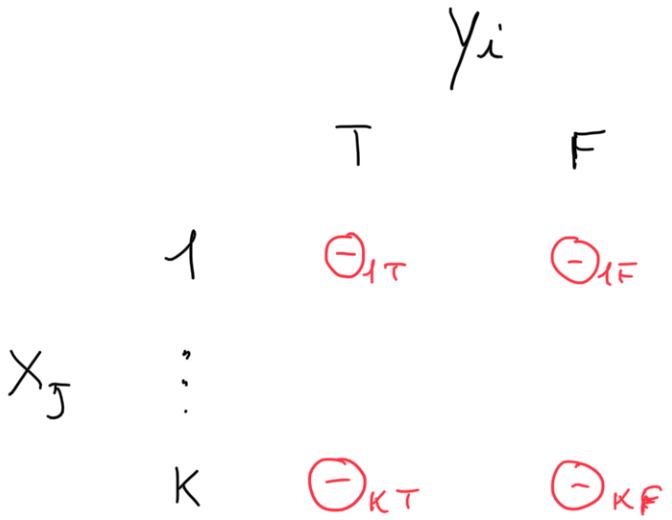
\includegraphics[width=0.5\textwidth]{images/parameterOfTheKthValueForYiClass.png}
    \caption{Parameter of the kth value for $y_i$ class. In this figure we assume $y_i$ is a binary class.}
    \label{fig:parameterOfTheKthValueForYiClass}
\end{figure}

In the formula there are too many expensive exponents. As result we take the log:
\begin{equation*}
    \log{f_i(\pmb{x})} = \sum_{k=1}^K N_{k \pmb{x}} \log{\theta_{k y_i}} + \log{(\frac{|\mathcal{D}_i|}{\mathcal{D}})}
\end{equation*}
Note that the term $\log{(\frac{|\mathcal{D}_i|}{\mathcal{D}})}$ is a scalar which does not depend on $x$. We can replace it with $w_0$ (bias). Moreover, we can define:
\begin{itemize}
    \item $\pmb{x}' = \begin{bmatrix} N_{1 \pmb{x}} \hdots N_{k \pmb{x}} \end{bmatrix}^T$ : vector of the number of times I have seen each feature (e.g. word in a document).
    
    \item $\pmb{w} = \begin{bmatrix} \log{\theta_{1 y_i}} \hdots \log{\theta_{k y_i}}\end{bmatrix}^T$
\end{itemize}

So, we can rewrite the above formula as:
$$\log{f_i(\pmb{x})} = \pmb{w}^T \pmb{x}' + w_0$$

Naive Bayes is a \textit{log-linear} model (as Gaussian distributions with shared $\Sigma$).